\documentclass[10pt,a4paper]{article}
%\documentclass[10pt,a4paper]{beamer}
\usepackage[utf8]{inputenc}
\usepackage{amsmath}
\usepackage{amsfonts}
\usepackage{amssymb}
\usepackage{graphicx}
\usepackage{subfigure}
\usepackage[left=2cm,right=2cm,top=2cm,bottom=2cm]{geometry}
\usepackage{kpfonts}
\usepackage[numbers]{natbib}
%other options include: round, curly, angle, or default options

\usepackage{media9}

\author{Zhixuan Cao}%\\ Advisor: Abani Patra}
\title{Towards Implementation of SPH in High Speed Compressible Flow Using Unequal Particle Mass}

\begin{document}

\maketitle
There are actually several options when using 
\section{•}
\section{Conservation of momentum and energy}
There are several factors which have significant impact on SPH (GSPH) simulation while using unequal particle mass. Such influence is more obvious for compressible flow, for which the density varies in a larger range.
In this section, the input parameters, including the left and right status are list in Table \ref{tab:1D-shock-input_parameters}. 
Sod shock tube test using unequal particle mass is test 2. Sod test using equal particle mass is test 7. Sjogreen test is test 5.

\subsection{Incorrect results using adaptive smoothing length and unequal particle mass }
The symmetric discretized formulation of SPH, Eq. (\ref{eq:ns-sph-v}) and Eq. (\ref{eq:ns-sph-e}), can guarantee strict conservation of momentum and energy \cite{monaghan1992smoothed} when smoothing length is uniform in the domain. However,
conservation property of SPH formulation loses when smoothing length varies. Unequal particle mass can lead to larger difference in smoothing length and make the situation worse, as shown in Fig. \ref{fig:Adapt-NoAdapt}.

\begin{figure}[!t]
\centering
\includegraphics[scale=0.35]{Figures/Adapt-NoAdapt}
\caption{The density distribution for modified Sod shock tube test. "SM" is short for using same particle mass. "DM" is short for using different particle mass. "AdptSml" represents using adaptive smoothing length. "NoAdptSml" means smoothing length keep constant. When particle mass is the same for all particles, correct result is obtained without adaptively changeing smoothing length. When we change smoothing length adaptively, an underestimation of density between shock front and contact discontinuity is observed, which is not surpring as nonuniform distribution of smoothing length breaks down conservation properties of SPH formulation. As for the case of unequal particle mass, even when the smoothing length is uniform, we still get incorrect results. Adaptively changing of smoothing length makes the result even worse.}
\label{fig:Adapt-NoAdapt}
\end{figure}

Even though using euqal particle mass without adaptively changing smoothing length gives us better match with analytic results. It is definitely not sufficient for real imeplementations. Because the solution of real problem is a complicated coupling of many different 1D problems. As will be shown in Fig. \ref{fig:Sjogreen-adptVSno}, adaptive smoothing length is required for getting correct solution even for some 1D tests (the Sjogreen's test). So we have to use adaptive smoothing length.

\begin{figure}[!htb]
    \centering
    \begin{minipage}{.495\textwidth}
        \centering
        \includegraphics[width=0.99 \textwidth]{./Figures/Sjogreen-adptVSno-d}
    \end{minipage}%
    \begin{minipage}{.495 \textwidth}
        \centering
        \includegraphics[width=0.99 \textwidth]{./Figures/Sjogreen-adptVSno-v}
    \end{minipage}%
    \\
    \begin{minipage}{.495\textwidth}
        \centering
        \includegraphics[width=0.99 \textwidth]{./Figures/Sjogreen-adptVSno-e}
    \end{minipage}%
    \begin{minipage}{.495 \textwidth}
        \centering
        \includegraphics[width=0.99 \textwidth]{./Figures/Sjogreen-adptVSno-p}
    \end{minipage}% 
    \caption{Sjogreen tests using uniform particle mass. "Adpt" refers to using adaptive smoothing length. "NO-Adpt" means without using adaptive smoothing length. When smoothing length is not adaptive, the results are obviously incorrect.}
    \label{fig:Sjogreen-adptVSno}
\end{figure}

\subsection{Improve results by adjusting parameters}
Before showing the correct way for fixing this problem. We present another way that can help us get correct results for "DM-AdaptSml" case in the previous paragraph. Better results obtained by adjusting parameter for adaptive smoothing length with the best match obtained by $\eta=1.5$. For "SM-AdaptSml" case, the numerical solution is much less sensitive to $\eta$, the the best numerical solution obtained around $\eta=1.3$. For other tests, we need to have another serials of trials to get good match with analytic solution. As we have already shown, such method helps to improve numerical solution but did not fix the issue. What's worse, there is no best choice for certain parameter in general sense.

\begin{figure}[!t]
\centering
\includegraphics[scale=0.35]{Figures/DM-Adpt-Etas}
\caption{An example of improving simulation results by adjusting parameter ($\eta$) for adaptive smoothing length : for "DM-AdaptSml" case. The plot shows density distribution for modified Sod shock tube test of a serials of several trials with different $\eta$. If a smaller $\eta$ used, the results become worse. Increasing $\eta$ from 1.0 to 1.3 and 1.5 helps to reduce the underestimation and the numerical solution gets closer to analytic solution. However, $\eta=2.0$ shows more underestimation of density between shock front and contact discontinuity, which means the best value for $\eta$ is around 1.5}
\label{fig:DM-Adpt-Etas}
\end{figure}

\begin{figure}[!t]
\begin{subfigure}
\centering
\includegraphics[scale=0.35]{Figures/EM-Adpt-Etas}
\end{subfigure}
\begin{subfigure}
\centering
\includegraphics[scale=0.35]{Figures/EM-Adpt-Etas_zoom}
\end{subfigure}
\caption{An example of improving simulation results by adjusting parameter ($\eta$) for adaptive smoothing length : for "EM-AdaptSml" case. The second plot is zoomed view of the first plot at region between shock and contact discontinuity. the best value for $\eta$ is around 1.3. Compared with case of uneuqal particle mass, the numerical solution for equal particle mass is less sensitive to parameter $\eta$}
\label{fig:EM-Adpt-Etas}
\end{figure}

Palying with different parameters manually can only help to get "good match" or "small variation" for test problems but useless for real implementation. However, such practice is common in test section for new SPH schemes \cite{monaghan1997sph, sigalotti2006shock}. More papers do not report details about manual parameter adjusting in their tests.

We can conclude that a rule of thrumb for choosing/developing robust techniques of SPH is that the technique has to be tested by comprehensive tests. For example, a comprehensive testing against all typical 1D problems is a good place to get start for compressible high speed compressible flow. However, it happens in some papers that new formulation was tested by one or two 1D problem and they concluded that the newly proposed method works well. Or in other cases, newly developed techniques are tested only by some 2D examples, where the analytic results is not available. And conclusion was drew based on some "looks similar" tests. Higher dimension, more complicated tests are definitely necessary but should be on a more solid basis of comprehensive 1D tests.
Another rule of thrumb for developing/choosing an useful technique for real implementation is that the technique has to be real adaptive. All parameters should be determined by simulation itself and there should no parameter adjusted manually by human for different test cases.

\subsection{Conservation formulation} \label{sec:Conservation-formulation}
The incorrect results are due to losing of strict linear momentum and energy conservation feature of original SPH formulation. \citet{evrard1988beyond} proposed to use mean of two interacting particles in place of original smoothing length to restore conservation feature of SPH formulation. Another way proposed by \citet{hernquist1989treesph} to restore momentum and energy conservation is using $0.5 \left( w_{ab}\left(h_a\right) + w_{ab}\left(h_b\right)\right)$ in place of $w_{ab}\left(h_a\right)$. 
We also propose an alternative formulation, which is similar to GSPH formulation \cite{inutsuka2002reformulation} in spirit. The corresponding discretized momentum equation of Euler equations by our way is:
\begin{equation}
\left\langle\dfrac{d \textbf{v}_a}{d t}\right\rangle = -\sum_b m_b \left(\dfrac{p_b}{\rho_b^2} \nabla_a w_{a b}\left(h_b\right) + \dfrac{p_a}{\rho_a^2} \nabla_a w_{a b}\left(h_a\right) + \frac{1}{2} \Pi_{ab}^{\beta} \left(\ \nabla_a w_{a b}\left(h_b\right) + \nabla_a w_{a b}\left(h_a\right)\right)\right) +\textbf{g} \label{eq:ns-sph-my-v}
\end{equation}
Discretized energy equation can be obtained in the same way.
\begin{equation}
\left\langle\dfrac{d e_a}{d t}\right\rangle = 0.5 \sum_b m_b \textbf{v}_{a b} \left(\dfrac{p_b}{\rho_b^2} \nabla_a w_{a b}\left(h_b\right) + \dfrac{p_a}{\rho_a^2} \nabla_a w_{a b}\left(h_a\right) + \frac{1}{2} \Pi_{ab}^{\beta} \left(\ \nabla_a w_{a b}\left(h_b\right) + \nabla_a w_{a b}\left(h_a\right)\right)\right) 
\label{eq:ns-sph-my-e}
\end{equation}

To summarize, the formulations that we tested are: 
\begin{itemize}
\item Classical SPH formulation (ME0):\\
The most commonly adopted formulation in classical SPH that claimed to be able to conserve momentum and energy.
\begin{align}
<\rho_a> = \sum_b m_b w_{ab} \left(h_b\right) \label{eq:ns-sph-d} \\
\left\langle\dfrac{d \textbf{v}_a}{d t}\right\rangle = -\sum_b m_b \left(\dfrac{p_a}{\rho_b^2} + \dfrac{p_b}{\rho_a^2} + \Pi_{ab}^{\beta} \right) \nabla_a w_{a b}\left(h_b\right) +\textbf{g} \label{eq:ns-sph-v} \\
\left\langle\dfrac{d e_a}{d t}\right\rangle=
 0.5\sum_b m_b \textbf{v}_{a b} \left(\dfrac{p_a}{\rho_b^2} + \dfrac{p_b}{\rho_a^2} + \Pi_{ab}^{\beta} \right) \cdot \nabla_a w_{a b}\left(h_b\right) \label{eq:ns-sph-e}
\end{align}
where, $a$ is the SPH particle index, $\textbf{v}_{a b} = \textbf{v}_a - \textbf{v}_b$.  $w_{a b}\left(h\right)$ is a concise form of $w\left(\textbf{x}_a - \textbf{x}_b, h\right)$.
\item Improvement proposed by \citet{evrard1988beyond} (ME2): \\
\begin{align}
<\rho_a> = \sum_b m_b w_{ab} \left(\frac{h_a+h_b}{2} \right) \label{eq:ns-sph-d-evrard} \\
\left\langle\dfrac{d \textbf{v}_a}{d t}\right\rangle = -\sum_b m_b \left(\dfrac{p_a}{\rho_b^2} + \dfrac{p_b}{\rho_a^2} + \Pi_{ab}^{\beta} \right) \nabla_a w_{a b}\left(\frac{h_a+h_b}{2}\right) +\textbf{g} \label{eq:ns-sph-v-evrard} \\
\left\langle\dfrac{d e_a}{d t}\right\rangle=
 0.5\sum_b m_b \textbf{v}_{a b} \left(\dfrac{p_a}{\rho_b^2} + \dfrac{p_b}{\rho_a^2} + \Pi_{ab}^{\beta} \right) \cdot \nabla_a w_{a b}\left(\frac{h_a+h_b}{2}\right) \label{eq:ns-sph-e-evrard}
\end{align}
\item Improvement proposed by \citet{hernquist1989treesph} (ME3):\\
\begin{align}
<\rho_a> = \sum_b m_b \frac{w_{ab}(h_a)+w_{ab}(h_b)}{2} \label{eq:ns-sph-d-hernquist} \\
\left\langle\dfrac{d \textbf{v}_a}{d t}\right\rangle = -\sum_b m_b \left(\dfrac{p_a}{\rho_b^2} + \dfrac{p_b}{\rho_a^2} + \Pi_{ab}^{\beta} \right) \nabla_a \left(
\frac{w_{ab}(h_a)+w_{ab}(h_b)}{2} \right) +\textbf{g} \label{eq:ns-sph-v-hernquist} \\
\left\langle\dfrac{d e_a}{d t}\right\rangle=
 0.5\sum_b m_b \textbf{v}_{a b} \left(\dfrac{p_a}{\rho_b^2} + \dfrac{p_b}{\rho_a^2} + \Pi_{ab}^{\beta} \right) \cdot \nabla_a \left(
\frac{w_{ab}(h_a)+w_{ab}(h_b)}{2} \right) \label{eq:ns-sph-e-hernquist}
\end{align}
\item Averaging first used in GSPH paper \citep{inutsuka2002reformulation} (ME4): \\
\begin{align}
<\rho_a> = \sum_b m_b \frac{w_{ab}(h_a)+w_{ab}(h_b)}{2} \label{eq:ns-sph-d-inutsuka} \\
\left\langle\dfrac{d \textbf{v}_a}{d t}\right\rangle = -\sum_b m_b \left( \left( \dfrac{p_a}{\rho_b^2} + 0.5 \Pi_{ab}^{\beta}\right) \nabla_a w_{a b}\left(h_b\right) + \left(\dfrac{p_b}{\rho_a^2}+ 0.5 \Pi_{ab}^{\beta}\right) \nabla_a w_{a b}\left(h_a\right) \right) +\textbf{g} \label{eq:ns-sph-v-inutsuka} \\
\left\langle\dfrac{d e_a}{d t}\right\rangle=
 0.5\sum_b m_b \textbf{v}_{a b} \left( \left( \dfrac{p_a}{\rho_b^2} + 0.5 \Pi_{ab}^{\beta}\right) \nabla_a w_{a b}\left(h_b\right) + \left(\dfrac{p_b}{\rho_a^2}+ 0.5 \Pi_{ab}^{\beta}\right) \nabla_a w_{a b}\left(h_a\right) \right) \label{eq:ns-sph-e-inutsuka}
\end{align}
\end{itemize}

We only show the effect of using these conservative formulations for test "SM-AdptSml". The effect on unequal particle mass cases will be discussed in later sections. We use all parameters the same as "SM-AdptSml" shown in Fig. \ref{fig:Adapt-NoAdapt}. As shown in Fig. \ref{fig:SM-Adapt-MEs}, the issue of density underestimation of orginal SPH formulation is solved by using these "averaged smoothing length" formulations. Among all these different average forms, the way proposed by \citet{evrard1988beyond} get best results for the modified Sod test, while other two ways also get pretty closer solution.

\begin{figure}[!t]
\centering
\includegraphics[scale=0.35]{Figures/SM-Adapt-MEs}
\caption{A comparison of different SPH formulations. All these averaged formulations get better results than orginal SPH. Among them, formulation proposed by \citet{evrard1988beyond} get best result. The newly proposed formulation  (see Eq. (\ref{eq:ns-sph-my-v})) shows almost the same result as that by  \citet{hernquist1989treesph}.}
\label{fig:SM-Adapt-MEs}
\end{figure}

\subsection{Numerical perturbation caused by averaging of smoothing length} \label{sec:Numerical-perturbation}
While averaged smoothing length restores the strict conservation feature of SPH formulation a numerical perturbation is also introduced simutaneously by the averaging.
Recall that the kernel function of particle $a$ has to be symmetric with repect to particle $a$. As a result, the gradient of kernel function at particle $a$ is anti-symmetric. Such anti-symmetric properties can guarantee the pressure gradient term, $\left(\dfrac{p_b}{\rho_b^2} + \dfrac{p_a}{\rho_a^2}\right) \nabla_a w_{a b}\left(h\right)$,  in momentum and energy equation (see Eq. (\ref{eq:ns-sph-v}) and (\ref{eq:ns-sph-e})) vanshes when pressure gradient is zero. However, it is obvious that the kernel function is unsymmetric when an averaged smoothing length is used. The gradient of kernel function is also not anti-symmetric any more as shown in Fig. \ref{fig:dw-ha}. The residual becomes non-zero. 
This non-zero residual can not be avoided in SPH formulation using averaged smoothing length and can induce perturbations in the solution. 
To minimize the effect of such perturbation, the smoothing length has to change smoothly. Sharp changes in smoothing length can induce significant perturbation which usually propagates in the domain and corrupts numerical solution. We take this into acccount when we develop a new method for smoothing length adaptivity. 
 
\begin{figure}[!t]
\centering
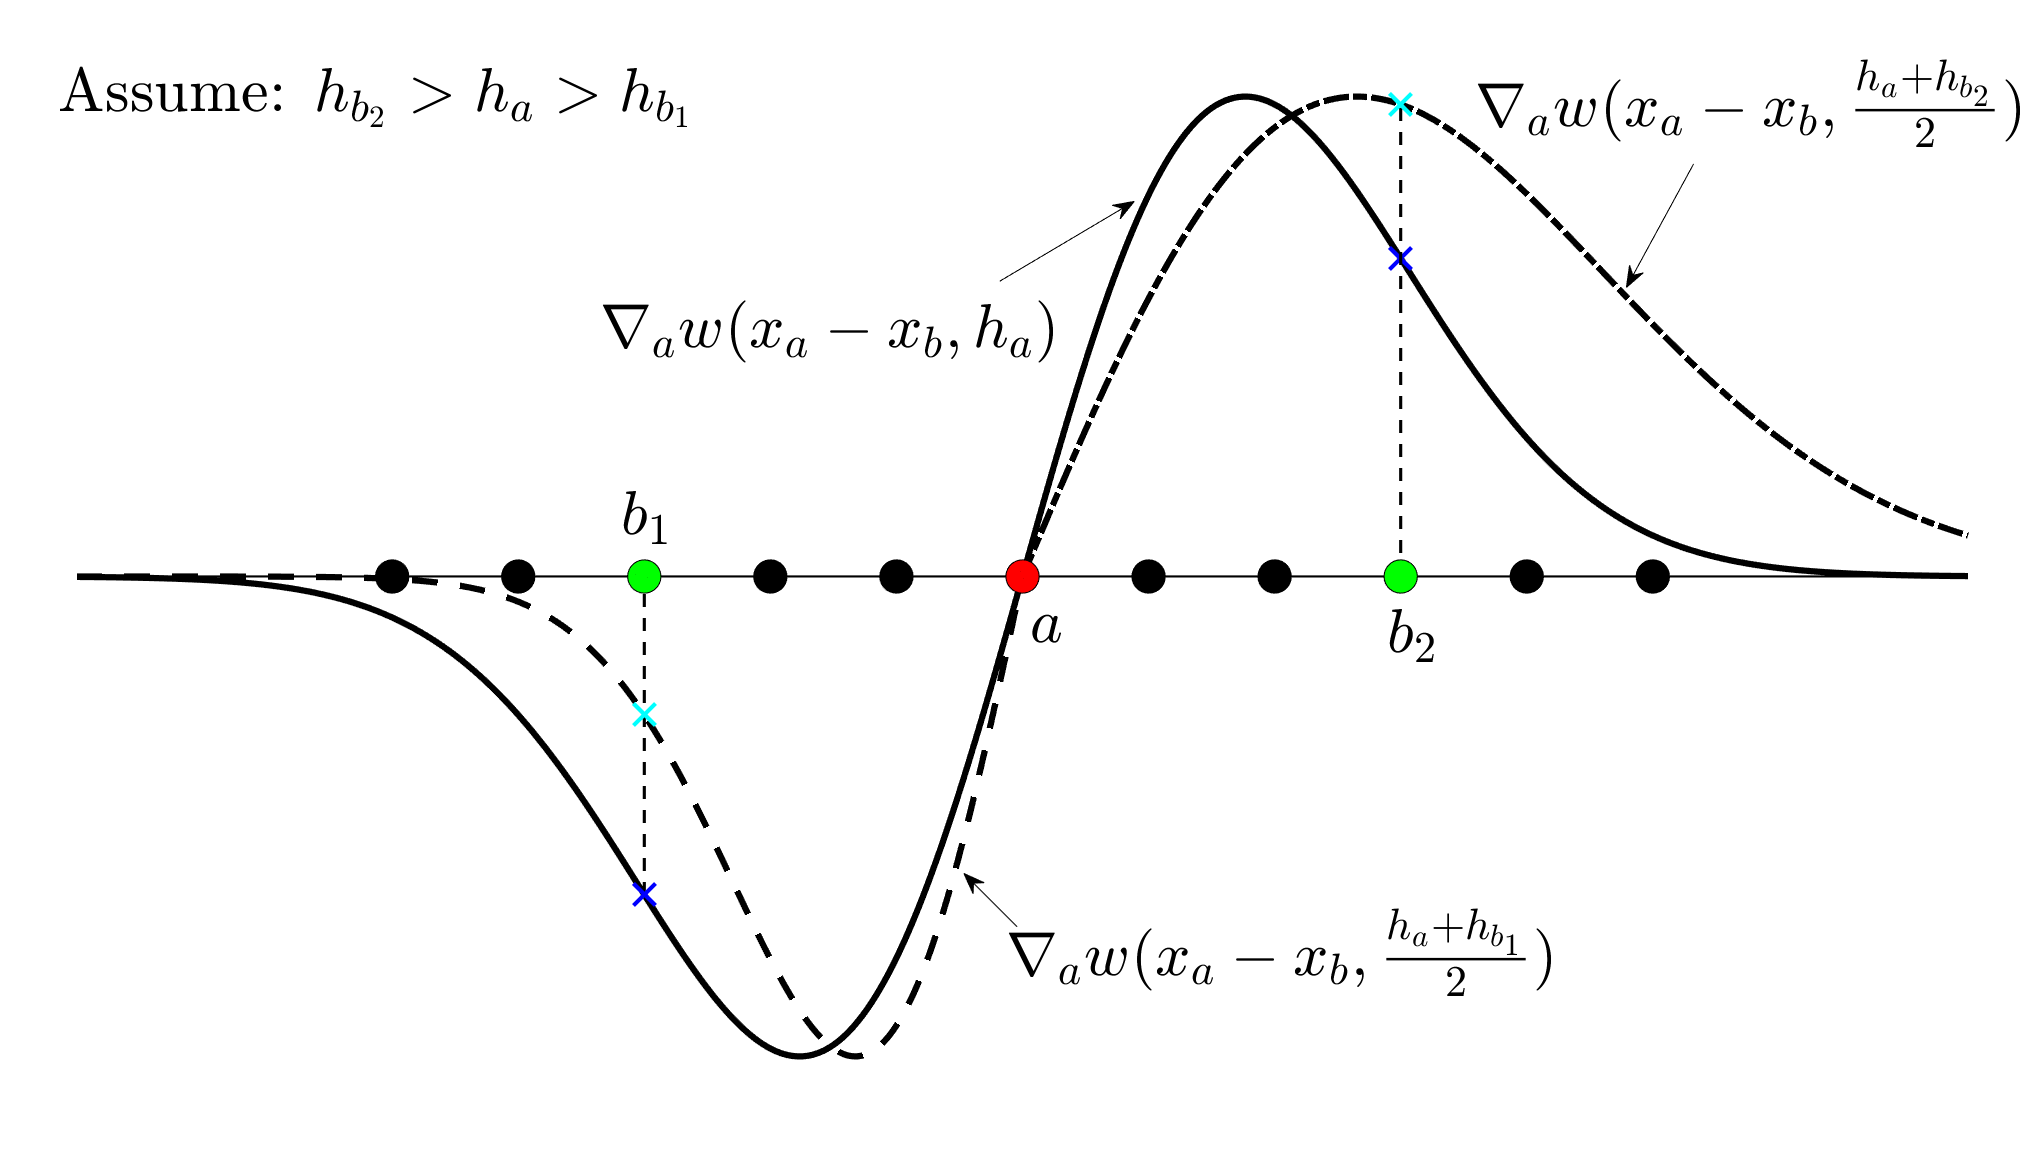
\includegraphics[scale=0.5]{Figures/dw-ha}
\caption{The gradient of kernel function becomes not anti-symmetric any more when using averaged smoothing length. For simplicity, we assume an uniform particle distribution. We also assume pressure, density and particle mass of all particles are equal. $-\dfrac{p_{b_1}}{\rho_{b_1}^2} \nabla_a w_{a b_1}\left(h_a\right) = \dfrac{p_{b_2}}{\rho_{b_2}^2} \nabla_a w_{a b2}\left(h_a\right)$ when $h=h_a$. However, the pressure term at symmetric position do not cancel out when averaged smoothing length is used, because $-\dfrac{p_{b_1}}{\rho_{b_1}^2} \nabla_a w_{a b_1}\left(\frac{h_a+h_{b_1}}{2}\right) < -\dfrac{p_{b_2}}{\rho_{b_2}^2} \nabla_a w_{a b2}\left(\frac{h_a+h_{b_1}}{2}\right)$. As a results a numerical perturbation is generated. Perturbation is generated in a similar mechanism in other two averaged smoothing length formulations.}    
\label{fig:dw-ha}
\end{figure}
We need to emphasize that, the perturbation can also been seen in 1D shock tube tests of all other papers, even though they are not as obvious as the one in our test. However, such perturbation was always ignored. In this section, we intentionally amplify such perturbation for discussion purpose. 
Of course, how significantly will such perturbation influence simulation results of real implementation is still an open question. 

To illustrate the existing and influence of such perturbation we create a sdiscontinuity of smoothing length intentionally near the left side boundary. As has been shown in Fig. \ref{fig:dw-ha}, the prerequirements of generating such perturbation are: 1) using averaged smoothing formulation, 2) smoothing length is nonuniform in space. A perturbation is created by assigning larger smoothing length to boundary ghost particles, see Fig. \ref{fig:Perturbation-ME2}.
The smoothing length of boundary ghost particles keep constant during simulation while smoothing length of real particles changes adaptively. Just like discontinuity of physical quantities (for example, the discontinuity at the middle of shock tube test), discontinuity in numerical resolution, the smoothing length, also induces a wave. A purteration can be observed clearly in the simulation result, starting near the left boundary and propagating into simulation domain. As shown in Fig. \ref{fig:Perturbation-ME0-tp1}, no such perturbation observed when using original SPH formulation (Eq. (\ref{eq:ns-sph-v}) and (\ref{eq:ns-sph-e})).
It needs to emphasize that such perturbation might be created unintentionally in implementation. Similar perturbation are observed when using averaged formulation proposed by \citet{hernquist1989treesph} and the new formulation propsed by us, see more details in appendix.

\begin{figure}[!t]
\centering
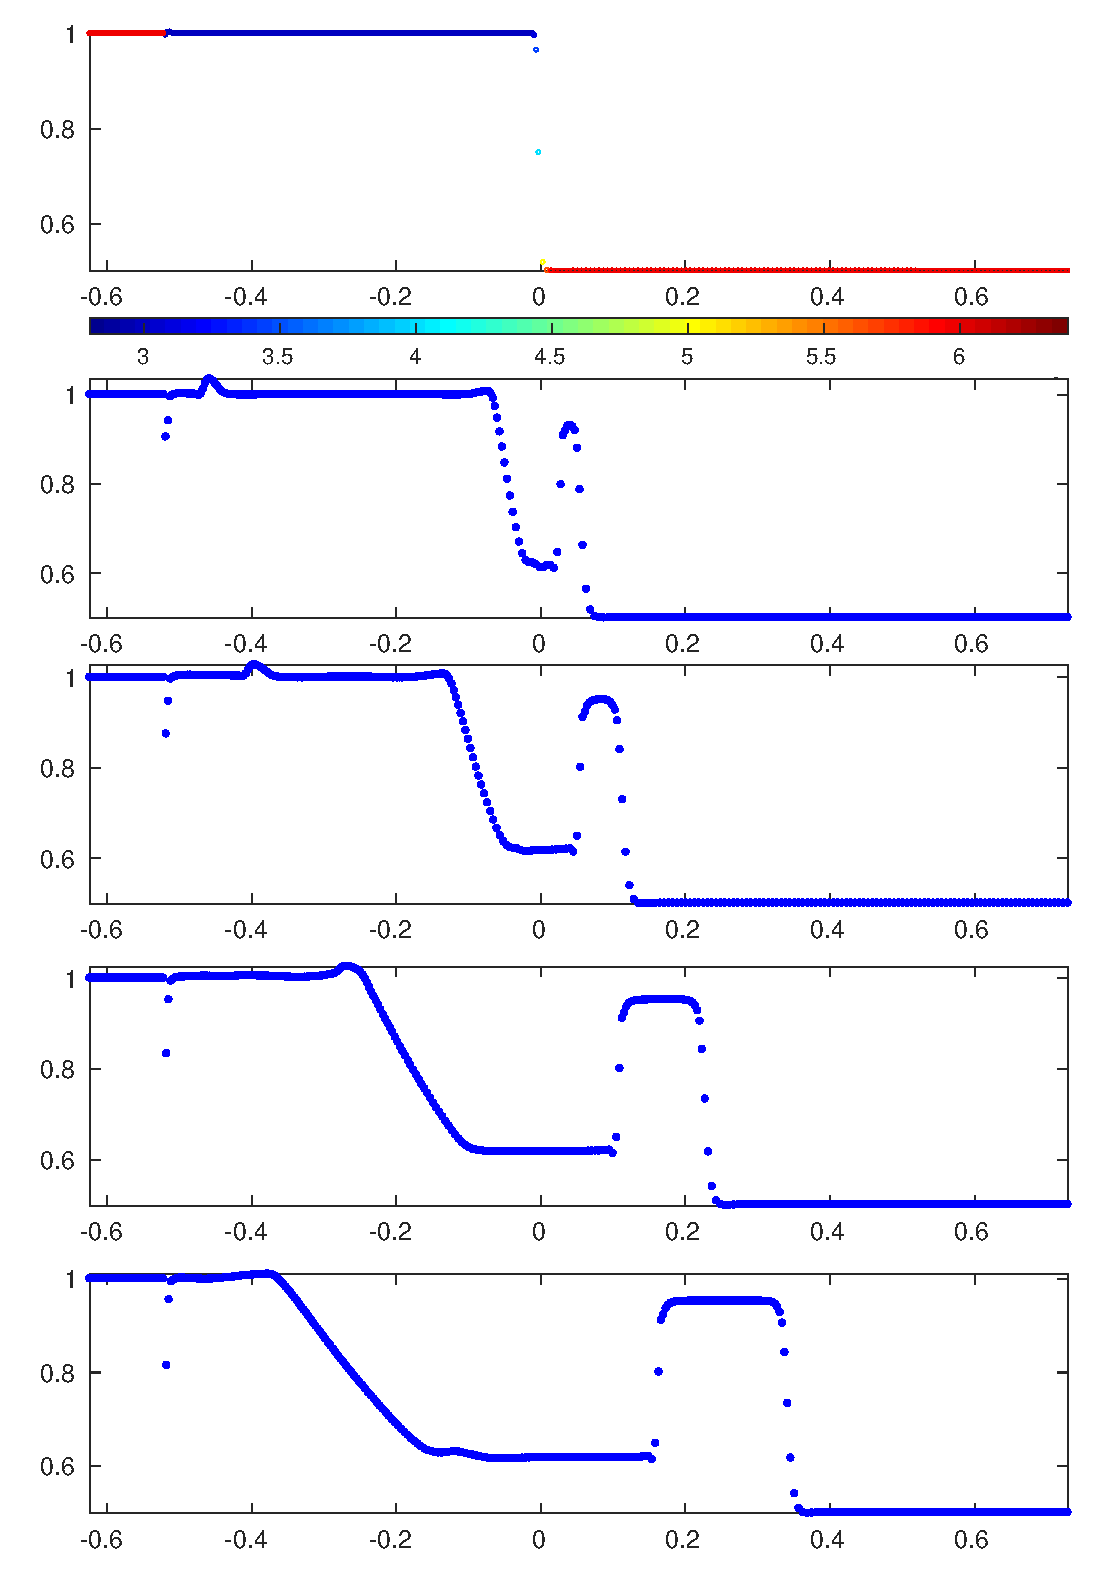
\includegraphics[scale=0.5]{Figures/Perturbation-ME2}
\caption{Plots of density as a function of location for modified Sod test at different time. The averaged SPH formulation by \citet{evrard1988beyond} is used. A numerical perturbation incepts near the left boundary and propogates into the domain. The first plot corresponding to t=0.001s, color map is for smoothing length. As shown in first plot, the smoothing length is discontinuous at the left boundary. Such discontinuity induces a numerical perturbation wave transporting towards right. The second plot to last one are corresponding to $t=0.05s$, $t=0.1s$, $t=0.2s$, $t=0.3s$ respectively. Actually, the smoothing length is also discontinuous at the middle. It should also induce another numerical perturbation. That perturbation has smaller magnitude but stll observable from the figure. It has the same propagating speed as the front of rarefaction. Both perturbations decays in time due to dissipation.}
\label{fig:Perturbation-ME2}
\end{figure}

\begin{figure}[!t]
\centering
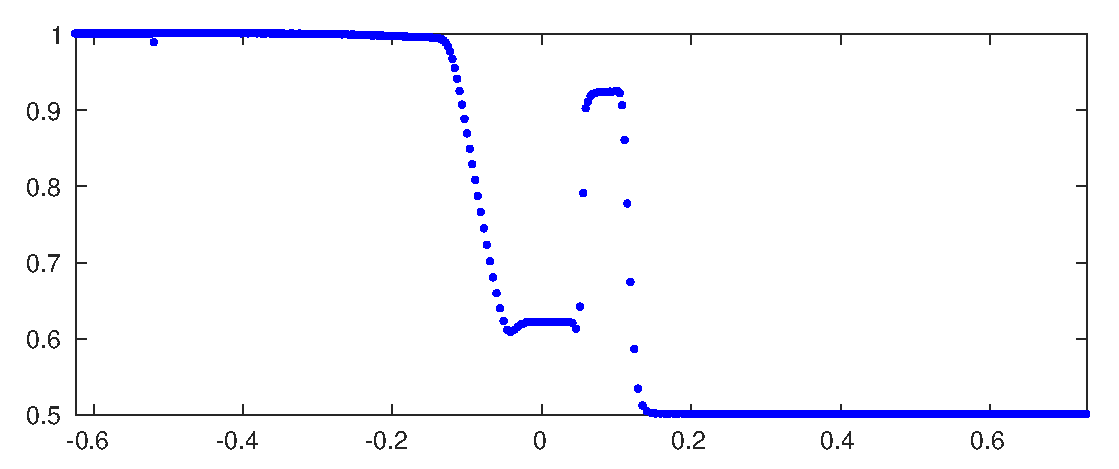
\includegraphics[scale=0.5]{Figures/Perturbation-ME0-tp1}
\caption{Density as a function of location for modified Sod test at t=0.1s. The original SPH formulation is used. Smoothing length is discontinuous at the left boundary. No numerical perturbation generated near the left boundary.}    
\label{fig:Perturbation-ME0-tp1}
\end{figure}

\subsection{Miss match of neighbouring}
Besides the numerical perturbation, another potential issue with averaged formulations is that relative larger pool of potential neighbours is required to guarantee actual conservation property of discretized conservation laws by SPH. It is offordable to treat all particles in the domain as potential neighbours for 1D tests. However, for large scale implementation, each particle should have its own neighbours which consist of a subset of all particles. It is the most efficent way in term of computation and storage to define neighbours as all particles within the support of the kernel function. However, conservation property of SPH formulation with averged smoothing length would lose when neighbours of each particle is defined in this way, as shown in Fig. \ref{fig:neigh_pool}.  
\begin{figure}[!t]
\centering
\includegraphics[scale=1.0]{Figures/neigh_pool}
\caption{This figure illustrates the situation where the strict conservation property of SPH lose even if the averaged smoothing length is used. In this figure, we assume that the neighbours of each particle is defined as the all particles within the support of kernel function whose radius is 3 times of smoothing length. When updating momentum, for example, of particle $a$, particle $c$'s contribution will be $m_c \left(\frac{p_c}{\rho_c^2}+\frac{p_a}{\rho_a^2}\right) \nabla_a w_{a c}\left(0.5(h_a+h_c)\right)$. However, when updating momentum of particle $c$, particle $a$ makes no contribution. That is to say, the momentum is not conserved in this case.} 
\label{fig:neigh_pool}
\end{figure}
%For example, in our implementation for simulating of volcanic plume \cite{gmd-2017-119}, the pool of neighbours is determined by the smallest externally tangent square of the kernel support which is a circle in 2D. Such strategy can simplify neighbour searching algorithm with the expense of more storage. It might be even more commom in SPH to choose interacting neighbours as memebers of pool of neighbours. 
Even though our discussion here is based on a specific example, the concept of such issue is general. 
%As the effects of this issue on simulation results are straight forward, no example simulation will be shown.
The source of "non-conservation" is obvious: particle $c$ is among neighbours of particle $a$ while partile $a$ is not a memember of particle $c$'s neighbours. Such miss-match of neighbour particles leads to losing of strict conservation. The idea to restore strict conservation is straight-forward: guarantee particle $a$ is also a neighbour of particle $b$ if particle $b$ is a neighbour of particle $a$. A well designed data structure might be able to achieve this pairly with acceptable computational cost. We will not investigate this option in this paper. An alternative solution is simply enlarging pool of neighbour particles. However, it is not as simple as it seems to be. The challenge not only comes from increase of computational cost due to extra time spending on searching for neighbours and accessing non-interacting neighbours. It is more difficult to adaptively decide an optimized pool size of neighbour particles, which can exclude "miss-match" while introduces mimnum waste of computation and memory. We will present our strategy to handle this issue in the next section.
For other two averaged formulation of SPH, a very similar mechanism (miss-match of neighbours) can also lead to losing of strict conservation. And the idea to fix it is the same.
\section{Adaptive smoothing length for unequal particle mass}
In previous section, we show that adaptive smoothing length is needed for real implementation but might generate incorrect results when particle mass is unequal. We then figure out that the source of the incorrectness is losing of strict conservation and proposed to use averaged smoothing length to get correct results. Then two potential issues associated with the averaged formulation is presented. we will propose an new smoothing adaptive method to relieve/avoid these two potential issues. 
\subsection{The gradient of particle mass distribution}
Our remedies of original adaptive smoothing length starts from treating the particle mass the same as other physical quantity as a function of location and time. The mass distributes uniformly over the computatinal domain when equal particle mass is used. When different masses are assigned to particles, the mass distribution is not a uniform function any more. Movement of particles also leads to change of mass distribution. 
The mass field (or mass distribution) over the computational domain can be evaluated using SPH interpolation based on discretized mass distribution.
\begin{equation}
<m\left(\textbf{x}\right)> \approx \sum_b m_b \dfrac{m_b}{\rho_b} w\left(\textbf{x}-\textbf{x}_b, h\right)
\label{eq:SPH-approximation-sum-mass}
\end{equation}
Recall that the kernel function satidfy the normalization condition. Equation (\ref{eq:SPH-approximation-sum-mass}) leads to $<m\left(\textbf{x}\right)>=m_b$ when all particles have the same mass.
The gradient of particle mass distribution is then evaluated naturely by: 
\begin{equation}
<\nabla m\left(\textbf{x}\right)>\approx
\sum_b m_b \dfrac{m_b}{\rho_b} \nabla w\left(\textbf{x} - \textbf{x}_b, h\right)
\label{eq:SPH-scalar-function-gradient-mass}
\end{equation}
When all particles have the same mass, Eq. (\ref{eq:SPH-scalar-function-gradient-mass}) leads to $<\nabla m\left(\textbf{x}\right)>=\textbf{0}$.
We can enlarge the smoothing length of particles with smaller mass and reduce the smoothing length of particles with larger mass to relieve the perturbation induced by sharp changes in smoothing length. 
The gradient of mass only indicates how fast the mass distribution change. It can not indicate whether the partcle mass at this location is smaller than masses  of surrounding particles or larger than masses of surrounding particles. Another property, mass distribution indicator is introduced:
\begin{equation}
<\chi\left(\textbf{x}\right)> \approx \sum_b \dfrac{(m_b-m)}{\rho_b} w\left(\textbf{x}-\textbf{x}_b, h\right)
\label{eq:SPH-mass-Indicator}
\end{equation}
The mass distribution indicator $<\chi\left(\textbf{x}\right)>$ has two properties, which can be easily infered from its definition.
\begin{itemize}
\item 
\begin{equation}
-1.0 \leqslant \chi \leqslant 1.0
\end{equation}
\item 
\begin{equation}  
\begin{cases} 
      \chi >0 & $Particle mass is smaller than that of surrounding particles on an average sense$ \\
      \chi <0 & $Particle mass is greater than that of surrounding particles on an average sense$ \\
\end{cases}
\label{eq:art-vis-shock}
\end{equation}
\end{itemize}

%Considering the gradient of particle mass is actually a vector. One natural way is to define kernel function on a elliptic support instead of a support of uniform radius in each direction for multi-dimension problems.
\subsection{Adaptive smoothing length based on particle mass gradient}
In section \ref{sec:Numerical-perturbation}, we demonstrated a numerical perturbation due to sharp changes of smoothing length. The formulation of adaptively changing smoothing length is based on the idea that smoothing length is propotional to $\left(\frac{m}{\rho}\right)^{1/d}$. Using the original adaptive smoothing length method as it is would lead to large difference in smoothing length among neighbouring particles if they have different particle mass. We propose a new method for adaptive smoothing length targeting at reducing smoothing  differences of length among neighbouring particles to relieve the numerical perturbation. In the new way of adaptively changing smoothing length, the coeffiecient $\sigma$ is not a constant. 
\begin{equation}
\sigma \left(\chi, \nabla m\right) =
\begin{cases}
\sigma_0 + \left(ln\left(\Theta+1\right)\right)^{0.5} & if \chi > 0 \\
\sigma_0 & Otherwise \\
\end{cases}
\label{eq:my-adaptive-sml-sigma}
\end{equation}
where  $\sigma_0 \sim 1$ is a constant. $\Theta$ is a variable calculated based on $\nabla m$. For 1D tests, we take $\Theta=\vert\nabla m\vert$. $\nabla m$ is a vector for higher dimension, we suggest to calculate $\nabla m$ according to 
\begin{equation}
\Theta =\frac{\sum_{i=1}^d \vert(\nabla^i m)\vert}{d}
\label{eq:my-adaptive-sml-Theta}  
\end{equation}
Equation (\ref{eq:my-adaptive-sml-sigma}) degenerate to the original equation, Eq (\ref{eq:adptive-sml-Gingold}) when particle mass is uniform. A larger coefficient $\sigma$ will be used for particles with smaller mass compared with its neighbours. The larger the gradient of mass distribution, the more we enlarge the coefficient $\sigma$. Such mechanism can adaptively reduce the difference of smoothing length between two neighboring particles.
It is necessary to mentioned that in this method, we do not change coefficient for particles with larger smoothing length. We also tried using a smaller coefficient $\sigma$ for particles with larger mass compared with its neighbours. But it tuned out to be a bad idea.
\subsection{Limit of smoothing length}
In this section, we made further modification on the method for smoothing length adjusting to avoid second issue associated with averaged formulation. We have to emphasize that it is just one possible solution for the "miss-match of neighbouring" issue by taking more partciles in the neighbour area as neighbours instead of only taking particles within the support of kernel function as neighbours. Another solution, which requires careful designed data structure and algorithm to make it affordable for real application, might also a promising method. 
As we mentioned, it is difficult to define to large enough pool of neighbours that can eliminate miss match of neighbouring, especially when there exist area with extremely small densities. The variation of particle mass makes the situation worse. 
Our solution to this challenge is setting an up-bound and lower bound to smoothing length by further modifying the adaptive smoothing length. The new formulation that sets limit on smoothing length is: 
\begin{equation}
h_a = (1-\lambda)\sigma \left(\chi, \nabla m\right) \left(\frac{m_a}{(1-\epsilon)\rho_a+\epsilon \rho_{a0}}\right)^{\frac{1}{d}}+ \lambda h_{a0}
\label{eq:my-adptive-sml-limit}
\end{equation}
where $\rho_0$ is initial density of particle $a$, $h_{a0}$ is initial smoothing length of particle $a$, $\lambda h_{a0}$ is the lower bound of smoothing length, $\epsilon$ is determined by the following equation.
\begin{equation}
\epsilon= \left( \frac{1-\lambda}{n-\lambda}\right)^d
\end{equation}
where the up-bound of smoothing length of particle $a$ is is set to $n$ times of intial smoothing length. The lower bound of smoothing length depends on coefficient $\lambda$ while the up-bound depends on $\epsilon$.
This new formulation will be consistent with Eq. \ref{eq:adptive-sml-Gingold} if we set lower bound as $0$ and up-bound as $\infty$ by setting $\lambda=0$ and $n=\infty$. 
In practice, the proper value for $n$ can be calibrated based on cavity flow test, where extremely small density formed. The recommended value for $n$ should be $10$ based on our tests. We take $\lambda=0=0.1$ in all of our tests. The Sjogreen's test is such problem.
\section{Numerical tests}
In this section we do comparisons between the new adaptive smoothing length method and original adaptive smoothing length method with a series of classical shock tube problems using unequal particle mass. Details in initial conditons, setting up of simulation, and comprehensive simulation results are provided to facilitate following up research and implementation.
We have an off topic remark regarding evaluating of any new techniques in SPH: bechmark testing based on partial tests can not evaluate the performance of the new technique comprehensively. Comprehensive testing is needed for any new technique before implementation. This is also the motivation that we do test our method with a series of typical shock tube tests.\\
\subsection{Tests setup}
Initial interval between any adjacent particles are equal. As a restult, particle mass is different if initial density is different. The intial density of some typical 1D tests are different. For other classical tests which has same density, we intentially set intial density be different so that all these tests are using different particle mass. Details of each tests can be found in Table \ref{tab:1D-shock-input_parameters}.

\begin{table}[htp]
\centering
      \caption{Overview of 1D shock tube tests}		
	  \begin{tabular}{lrrrrrrrrrrrr}
	    \hline
	          & $\rho_L$ & $p_L$ &$v_L$ & $\rho_R$ & $p_R$ &$v_R$ & $\Delta x_L$ & $\Delta x_R$  & $[x_L, x_R]$ & $m_L$ & $m_R$ & $t_f$\\
	    \hline
	    Test 1 & $1.0$ & $1.0$ &$0$ & $0.5$ & $0.2$ &$0$ & $0.003$ & $0.003$  & $[-0.4, 0.4]$ & $0.003$ & $0.0015$ & $0.2$\\
	    Test 2 & $1.0$ & $1.0$ &$0$ & $0.25$ & $0.1795$ &$0$ & $0.003$ & $0.003$  & $[-0.4, 0.4]$ & $0.003$ & $0.00075$ & $0.17$\\
	    	Test 3 & $2.0$ & $1.95$ &$1.0$ & $1.0$ & $1.95$ &$-1.0$ & $0.003$ & $0.003$  & $[-0.4, 0.4]$ & $0.006$ & $0.003$ & $0.13$\\
	    Test 4 & $1.0$ & $2.4$ &$8.0$ & $0.5$ & $0.4$ &$-0.25$ & $0.003$ & $0.003$  & $[-0.4, 0.4]$ & $0.003$ & $0.0015$ & $0.05$\\
	    	Test 5 & $1.0$ & $-2.0$ &$0.4$ & $1.0$ & $0.4$ &$2.0$ & $0.003$ & $0.003$  & $[-0.4, 0.4]$ & $0.003$ & $0.003$ & $0.18$\\
	    	Test 6 & $1.0$ & $0$ &$1000$ & $1.0$ & $0$ &$0.01$ & $0.003$ & $0.003$  & $[-0.5, 0.5]$ & $0.003$ & $0.003$ & $0.01$\\
	    	Test 7 & $1.0$ & $1.0$ &$0$ & $0.25$ & $0.1795$ &$0$ & $0.00075$ & $0.003$ & $[-0.4, 0.4]$ & $0.00075$ & $0.00075$ & $0.17$\\
	    \hline
	  \end{tabular}
	  \label{tab:1D-shock-input_parameters}
\end{table}
Where, subscript $L$ refers left side and $R$ for right side. $\Delta x$ is interval between two adjcent particles. $m$ is particle mass. $t_f$ is the time to terminate simulation and ploting the results. Please be aware of the fact that in our plots for shock tube tests, the x axis is normalized by time, that is $x/t_f$.
Test 1 consists of a left rarefaction, a right travelling contact and a right shock. Density decreases at down wind of contact wave.
Test 2 also consists of a left rarefaction, a right travelling contact and a right shock. Density increases at down wind of contact wave.
Test 3 is a double expansion test with different initial dnesity.
Test 4 is a double shock tests with different initial density on the right side and left side.
Test 5 and Test 6 are two extreme cases. Test 5 is a cavity flow while test 6 is a strong blast flow.


%\subsection{Calibration of $\sigma_0$}
%$\sigma_0$ in Eq. (\ref{eq:my-adaptive-sml-sigma}) should be around $1.0$. In this section, we discuss the influence of value of $\sigma_0$. It turned out that $\sigma_0~1.1$ can generate best results for all test cases. 
%\subsection{Density updating in SPH}

\subsection{Tests results}
Three different conservative (averaged) SPH formulations using the new adaptive smoothing length method are compared against the conservative SPH formulations using classical adaptive smoothing length method in this section.
The density, velocity and internal energy of all tests are plot in Fig. (\ref{eq:Dirac-translation}). The $x$ axis of all these plots are $x/t_{end}$. Zoomed views are provided to illustrate the numerical fluctuations at front of shock waves or rarefactions. Such fluctuations can be observed in plots for all physical quantities. We only show zoomed view of one example fluctuation for each test case. We also presented zoomed view around the contact discontinuities, where large fluctuations shows up. Such fluctuation can be observed in results reported by others using equal particles mass.
 
In theses plots, "ME2" refers to formulations proposed by \citet{evrard1988beyond}. "ME3" refers to formulations proposed by \citet{hernquist1989treesph}, "ME4" refers to the formulation that we proposed.

\begin{figure}[!htb]
    \centering
    \begin{minipage}{.325\textwidth}
        \centering
        \includegraphics[width=0.99 \textwidth]{./Figures/Results_OnlyAdpt_SmallP/GSPH-Sod-NewAdpt-OldAdpt-rho}
    \end{minipage}%
    \begin{minipage}{.325 \textwidth}
        \centering
        \includegraphics[width=0.99 \textwidth]{./Figures/Results_OnlyAdpt_SmallP/GSPH-Sod-NewAdpt-OldAdpt-v}
    \end{minipage}%
    \begin{minipage}{.325 \textwidth}
        \centering
        \includegraphics[width=0.99 \textwidth]{./Figures/Results_OnlyAdpt_SmallP/GSPH-Sod-NewAdpt-OldAdpt-e}
    \end{minipage}%
    \\
    \begin{minipage}{.325\textwidth}
        \centering
        \includegraphics[width=0.99 \textwidth]{./Figures/Results_OnlyAdpt_SmallP/GSPH-Sod-NewAdpt-OldAdpt-rho-zoom1}
    \end{minipage}%
    \begin{minipage}{.325 \textwidth}
        \centering
        \includegraphics[width=0.99 \textwidth]{./Figures/Results_OnlyAdpt_SmallP/GSPH-Sod-NewAdpt-OldAdpt-v-zoom}
    \end{minipage}%
    \begin{minipage}{.325 \textwidth}
        \centering
        \includegraphics[width=0.99 \textwidth]{./Figures/Results_OnlyAdpt_SmallP/GSPH-Sod-NewAdpt-OldAdpt-e-zoom}
    \end{minipage}%    
    \caption{Plots of density, velocity and internal energy for test 1. Plots on the second row are zoomed view of density in front of right shock, zoomed view of velocity in the region between right shock and middle contact and zoomed view of specific internal energy at the middle contact respectively. Old way of adaptive smoothing length introduces fluctuations in region far away from shock front while the the new way for smoothing length adaprivity eliminated such fluctuations completely. And it is obvious that such fluctuation is due to adaptive smoothing length and has nothing to do with different conservative formulations. The zoomed view of velocity illustrates that "ME2" obtains least error compared with other two formulations.}
    \label{fig:GSPH-sod-NewAdpt-OldAdpt}
\end{figure}

The third zoomed view in Fig. \ref{fig:GSPH-sod-NewAdpt-OldAdpt} shows that the new way of smoothing length adaptivity does not reduce fluctuations around the contact for this test. We have to mention that such fluctuation exist in other tests using equal particle mass. And the source of such fluctuation is possibly caused by sharp change in smoothing length due to sharp change of density, whose mechanism has been illustrated in Fig. \ref{fig:dw-ha} As our focus here is to address issues associated with unequal particle mass, it is acceptable if our new smoothing length adaptivity method does not eliminate fluctuations of internal energy caused by sources other than unequal particle mass. Nevertheless, the new method does help reduce the fluctuations around contact discontinuities for other tests.

\begin{figure}[!htb]
    \centering
    \begin{minipage}{.325\textwidth}
        \centering
        \includegraphics[width=0.99 \textwidth]{./Figures/Results_OnlyAdpt_SmallP/Sod-NewAdpt-OldAdpt-rho}
    \end{minipage}%
    \begin{minipage}{.325 \textwidth}
        \centering
        \includegraphics[width=0.99 \textwidth]{./Figures/Results_OnlyAdpt_SmallP/Sod-NewAdpt-OldAdpt-v}
    \end{minipage}%
    \begin{minipage}{.325 \textwidth}
        \centering
        \includegraphics[width=0.99 \textwidth]{./Figures/Results_OnlyAdpt_SmallP/Sod-NewAdpt-OldAdpt-e}
    \end{minipage}%
    \\
    \begin{minipage}{.325\textwidth}
        \centering
        \includegraphics[width=0.99 \textwidth]{./Figures/Results_OnlyAdpt_SmallP/Sod-NewAdpt-OldAdpt-rho-zoom1}
    \end{minipage}%
    \begin{minipage}{.325 \textwidth}
        \centering
        \includegraphics[width=0.99 \textwidth]{./Figures/Results_OnlyAdpt_SmallP/Sod-NewAdpt-OldAdpt-rho-zoom2}
    \end{minipage}%
    \begin{minipage}{.325 \textwidth}
        \centering
        \includegraphics[width=0.99 \textwidth]{./Figures/Results_OnlyAdpt_SmallP/Sod-NewAdpt-OldAdpt-e-zoom2}
    \end{minipage}%    
    \caption{Plots of density, velocity and internal energy for test 2. Plots on the second row are zoomed view of internal energy in front of left rarefaction, zoomed view of density around middle contact and zoomed view of internal energy at the middle contact respectively. The first zoomed view again illustrates the elimination of fluctuations by the new way for smoothing length adaprivity. The second and third zoomed view shows that fluctuation in density around the contact discontinuity is smoothed out by new way for smoothing length adaptivity while the fluctuation of internal energy is not eliminated.}
    \label{fig:Sod-NewAdpt-OldAdpt}
\end{figure}

\begin{figure}[!htb]
    \centering
    \begin{minipage}{.325\textwidth}
        \centering
        \includegraphics[width=0.99 \textwidth]{./Figures/Results_OnlyAdpt_SmallP/d-exp-NewAdpt-OldAdpt-rho}
    \end{minipage}%
    \begin{minipage}{.325 \textwidth}
        \centering
        \includegraphics[width=0.99 \textwidth]{./Figures/Results_OnlyAdpt_SmallP/d-exp-NewAdpt-OldAdpt-v}
    \end{minipage}%
    \begin{minipage}{.325 \textwidth}
        \centering
        \includegraphics[width=0.99 \textwidth]{./Figures/Results_OnlyAdpt_SmallP/d-exp-NewAdpt-OldAdpt-e}
    \end{minipage}%
    \\
    \begin{minipage}{.325\textwidth}
        \centering
        \includegraphics[width=0.99 \textwidth]{./Figures/Results_OnlyAdpt_SmallP/d-exp-NewAdpt-OldAdpt-v-zoom}
    \end{minipage}%
    \begin{minipage}{.325 \textwidth}
        \centering
        \includegraphics[width=0.99 \textwidth]{./Figures/Results_OnlyAdpt_SmallP/d-exp-NewAdpt-OldAdpt-e-zoom}
    \end{minipage}%
    \begin{minipage}{.325 \textwidth}
        \centering
        \includegraphics[width=0.99 \textwidth]{./Figures/Results_OnlyAdpt_SmallP/d-exp-NewAdpt-OldAdpt-e-zoom2}
    \end{minipage}%    
    \caption{Plots of density, velocity and internal energy of test 3. Plots on the second row are zoomed view of velocity in front of left rarefaction, zoomed view of specific internal energy in front of middle contact (travels left) and zoomed view of specific internal energy behind middle contact respectively. Old way of adaptive smoothing length introduces fluctuations in region far away from wave front while the the new way for smoothing length adaprivity eliminated such fluctuations.}
    \label{fig:d-exp-NewAdpt-OldAdpt}
\end{figure}

\begin{figure}[!htb]
    \centering
    \begin{minipage}{.325\textwidth}
        \centering
        \includegraphics[width=0.99 \textwidth]{./Figures/Results_OnlyAdpt_SmallP/d-shock-NewAdpt-OldAdpt-rho}
    \end{minipage}%
    \begin{minipage}{.325 \textwidth}
        \centering
        \includegraphics[width=0.99 \textwidth]{./Figures/Results_OnlyAdpt_SmallP/d-shock-NewAdpt-OldAdpt-v}
    \end{minipage}%
    \begin{minipage}{.325 \textwidth}
        \centering
        \includegraphics[width=0.99 \textwidth]{./Figures/Results_OnlyAdpt_SmallP/d-shock-NewAdpt-OldAdpt-e}
    \end{minipage}%
    \\
    \begin{minipage}{.325\textwidth}
        \centering
        \includegraphics[width=0.99 \textwidth]{./Figures/Results_OnlyAdpt_SmallP/d-shock-NewAdpt-OldAdpt-rho-zoom2}
    \end{minipage}%
    \begin{minipage}{.325 \textwidth}
        \centering
        \includegraphics[width=0.99 \textwidth]{./Figures/Results_OnlyAdpt_SmallP/d-shock-NewAdpt-OldAdpt-e-zoom}
    \end{minipage}%
    \begin{minipage}{.325 \textwidth}
        \centering
        \includegraphics[width=0.99 \textwidth]{./Figures/Results_OnlyAdpt_SmallP/d-shock-NewAdpt-OldAdpt-v-zoomed}
    \end{minipage}%    
    \caption{Plots of density, velocity and internal energy of test 4. Surprisely, "ME3" and "ME4" generate incorrect results for this test. Plots on the second row are zoomed view of density around the left shock, zoomed view of specific internal energy around middle contact and zoomed view of velocity between two shocks respectively. We do not show any zoomed view about it even fluctuations in the region not reached by waves does exist. The last zoomed view shows that our new smoothing adaptivity method introduces fluctuation of velocity between two shocks while calssical method does not.}
    \label{fig:d-shock-NewAdpt-OldAdpt}
\end{figure}

As shown in zoomed view of simulation results, the original method for adaptive smooth length can introduce numerical fluctuations in the domain where the waves have not propagated into yet. Such fluctuation always exists no matter which formulation we choose for "averaging smoothing length". It has been shown that the numerical fluctuations in all tests are eliminated by the adopting the new adaptive smoothing length method. In addition, the large fluctuations around contact wave are also reduced by the new smoothing length adaptive method. Such fluctuations can be also seen in shock tube tests using equal particle mass. To the best of the author's knowledge, there is no paper addresses such fluctuation yet. Among these three different conservative formulations, the formulation proposed by \citet{evrard1988beyond} gives best results. Other two formulations give incorrect results for double shock tests even thought they work pretty well for any other tests, which reminds us that comprehensive tests is really necessary for any newly proposed technique. 
%It is also very interesting to to see whether incorrect results will be obtained if equal particle mass is used.
Extra attention should be paid to any possible limitation of any new technique if the tests in papers are not comprehensive.
We have to point out one limitation of our tests presented here: the particle mass is not randomly different. As we have mentioned in previous section, the differece in particles mass are created by assign equal interval between particles. We only have one "discontinuity" in particle mass distribution. In higher dimensional implementations of unequal particle mass, situation is more complicated.
\bibliographystyle{plainnat}
\bibliography{../Reference}
\end{document}